% % % Set the style for this file:
\pagestyle{standard}

% % % Beginning of the chapter
\chapter{Notions of infrared thermography}\label{chapter1}

	% % % Set the style for the first page:
	\thispagestyle{chapter-first-page}
	
	\section{Infrared Thermography. Infrared radiation spectrum.}\label{section1.1}
	
		Infrared thermography (IRT) is a science dedicated to the acquisition and processing of thermal information from non-contact measurement devices. Infrared measuring devices acquire infrared radiation emitted by an object and transform it into an electronic signal. As a non-contact technique, IRT has some advantages in relation to other techniques for temperature measurement. For example, the temperature of extremely hot objects or dangerous products, such as acids, can be measured safely, keeping the user out of danger. It also provides protection for the object under investigation since there is no need to attach any temperature measuring device to it, which makes it much less invasive.
		
		Infrared (IR) radiation is the energy irradiated by a surface that has a temperature above the absolute zero \ref{ref2}. Within the electromagnetic spectrum, IR radiation is defined as the radiation band that spans from 0.75 $\mu$m to 1000 $\mu$m in wavelength (Figure \ref{fig1.1}). Much of the IR spectrum, however, is generally avoided for IRT applications due to atmospheric absorption. This absorption occurs mainly with H$_{2}$O and CO$_{2}$ molecules as they are well known for being good heat absorbers (Figure \ref{fig1.2}). According to this fact, the IR wavelength range is sometimes further divided into 5 additional categories:

		\begin{enumerate}[label={\Roman*.}]
			\item Near-infrared (NIR) from 0.75 $\mu$m to 1.4 $\mu$m.
			\item Short-wavelength infrared (SWIR) from 1.4 $\mu$m to 3 $\mu$m.
			\item Mid-wavelength infrared (MWIR) from 3 $\mu$m to 8 $\mu$m.
			\item Long-wavelength infrared (LWIR) from 8 $\mu$m to 15 $\mu$m.
			\item Far infrared (FIR) from 15 $\mu$m to 1000 $\mu$m.
		\end{enumerate}
		
		\begin{figure}[ht!]
			\centering
			\captionsetup{justification=centering,margin=2cm}
			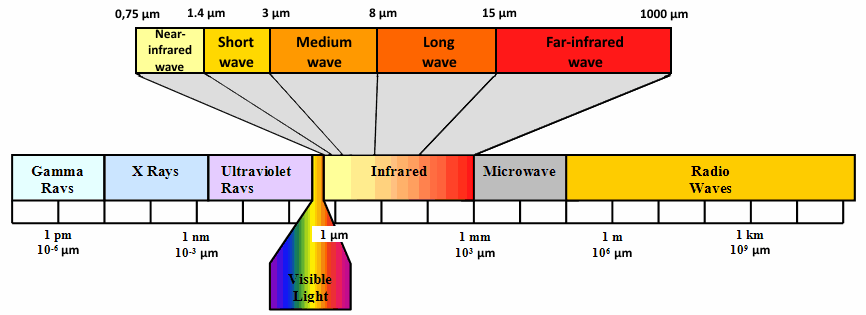
\includegraphics[scale=0.75]{Figures/Chapter01/Spectrum-of-electromagnetic-radiation.png}
			\caption{Electromagnetic spectrum showing the portion corresponding to IR radiation.}\label{fig1.1}
		\end{figure}
		
		It is important to note that this classification is somewhat arbitrary and therefore can vary within literature. Most IR sensors are designed to work in the LWIR part of the spectrum since this is the range that minimizes these absorptions. In this study, as we use an IR camera sensitive only to the fourth type, we will refer to IR as the LWIR except otherwise explicitly stated.
				
		\begin{figure}[ht!]
			\centering
			\captionsetup{justification=centering,margin=2cm}
			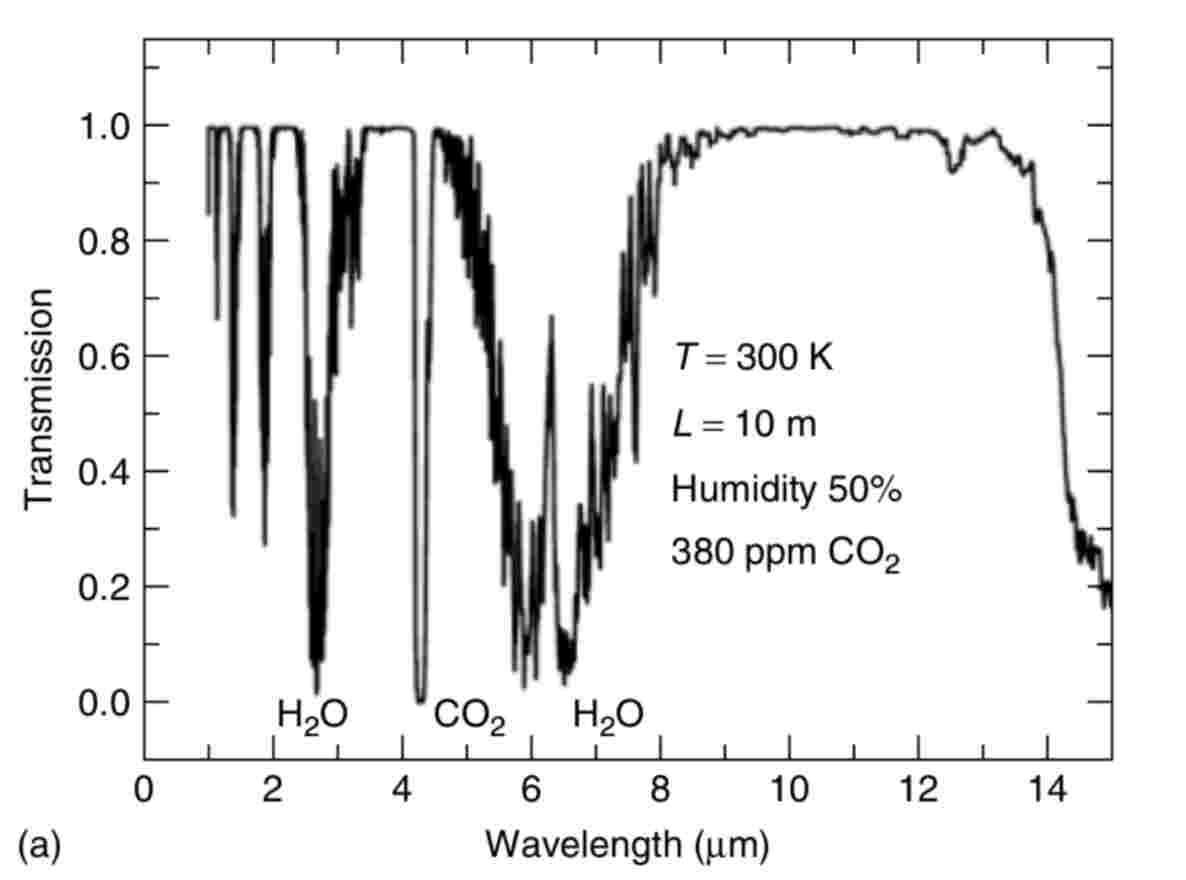
\includegraphics[scale=0.35]{Figures/Chapter01/Transmission.jpg}
			\caption{An example of atmospheric transmission plot for infrared radiation. For some of the minima we can see the molecule responsible for the absorption.}\label{fig1.2}
		\end{figure}
		
		There are, of course, some caveats associated with the use of IRT. One of them is in fact related with its advantageous characteristic of being a non-contact technique: IR radiation has to travel some distance from the target surface to the infrared sensor passing through some media that can either let it pass almost completely or strongly attenuate it. Using vacuum would solve this particular issue but sometimes it's not possible to perform infrared measurements in vacuum. Additional complications are related with the intrinsic characteristics of the emitting material and the IR sensor's particular response to IR radiation. All these factors need to be "compensated" in order to obtain meaningful quantitative IR measurements. We will discuss the most important ones in the following sections.
		
	\section{Plank's law for blackbodies. IR radiation dissipation.}\label{section1.2}
	
		According to Planck’s law, the IR emissive power ($N$) of a blackbody\footnote{{\footnotesize A blackbody is an idealized physical body that absorbs all incident electromagnetic radiation, regardless of frequency or angle of incidence.}} at a temperature $T$, with a wavelength between $\lambda$ and $\lambda+d\lambda$ is given by Equation \ref{eq1.1}, where C$_{1}$ ($2hc^2$) and C$_{2}$ ($hc/k_{B}$) are constant, often called first and second radiation constants respectively \ref{ref3}.
		
		\begin{equation}\label{eq1.1}
			N_{b}(\lambda,T)d\lambda=\frac{C_{1} \cdot \lambda^{-5}}{\exp (\frac{C_{2}}{\lambda\cdot T}) -1} d\lambda
		\end{equation}\bigskip
		
		Here the subindex $b$ denotes the special case of the blackbody. Figure \ref{fig1.3} shows this functional dependence in terms of an equivalent magnitude (monochromatic\footnote{{\footnotesize Monochromatic here refers to “per wavelength interval”. Also referred to as “spectral”.}} irradiance) for six different temperatures \ref{ref4}. The gray line represents the displacement of the maximum for each temperature. Note that, as the temperature decreases, the maximum emissive power moves to higher wavelengths, this is known as the Wien’s displacement law \ref{ref5}.
		
		There are three ways by which the incoming emissive power may be dissipated: absorption, transmission and reflection \ref{ref6}. The fractions of the total radiant energy that are associated with each of these modes of dissipation are referred to as the \textit{absorptivity}, \textit{transmissivity} and \textit{reflectivity} of the body. Three parameters are used to describe these phenomena: the spectral absorptance $\alpha$, which is the fraction of the spectral emissive power absorbed by the object, the spectral reflectance $\rho$, which is the fraction of the spectral emissive power reflected by the object, and the spectral transmittance $\tau$, which is the fraction of the spectral emissive power transmitted by the object.
		
		\begin{figure}[ht!]
			\centering
			\captionsetup{justification=centering,margin=2cm}
			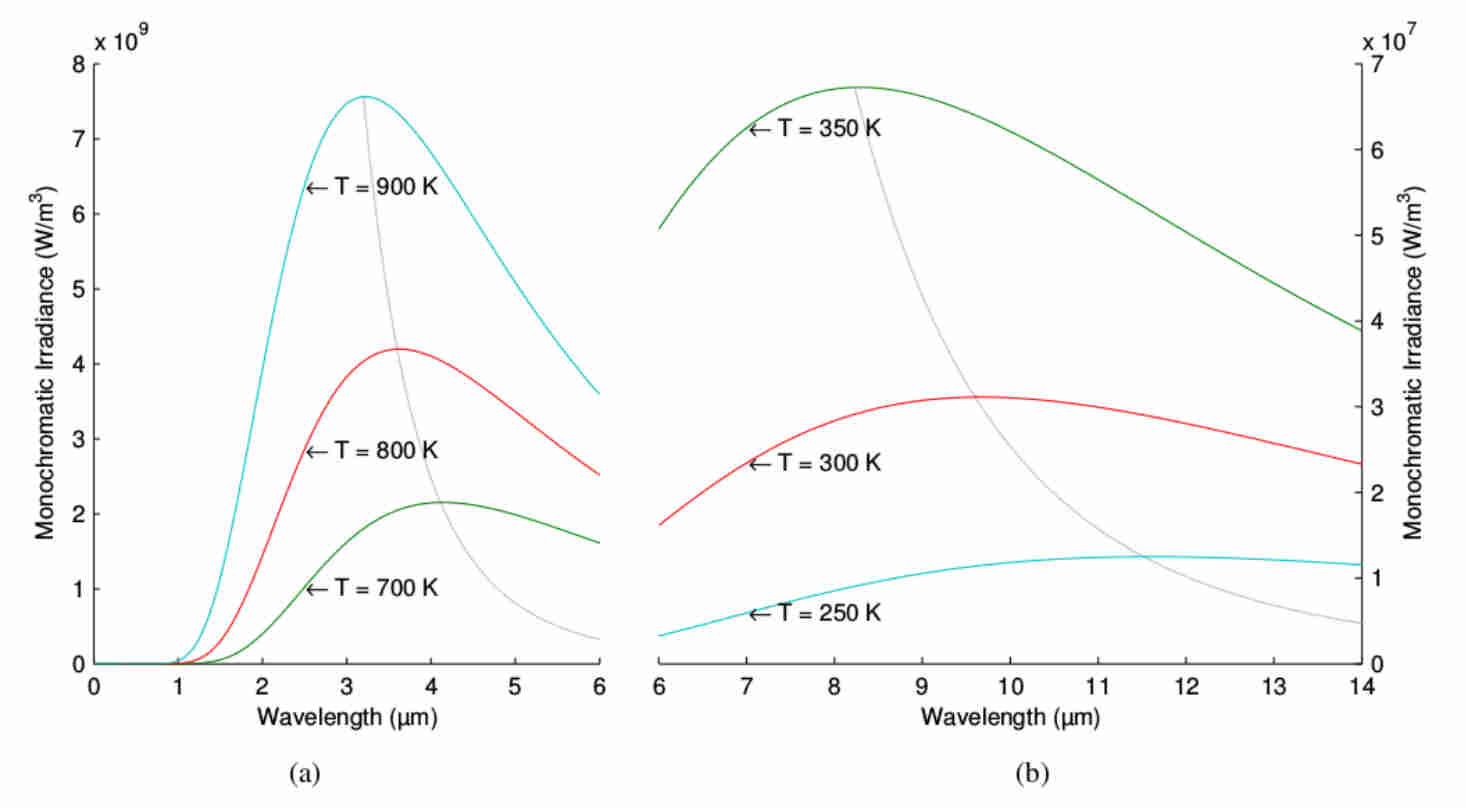
\includegraphics[scale=0.35]{Figures/Chapter01/PlankFunction.jpg}
			\caption{Planck’s law in terms of the  monochromatic irradiance of  a blackbody in thermal equilibrium at a definite temperature. (a) Objects with a high temperature emit most of the radiation in the middle wave infrared; (b) Objects with a low temperature emit most of the radiation in the long wave infrared. The two parts of the graph are scaled differently on the y-axis.}\label{fig1.3}
		\end{figure}		
		
		These three parameters are, in general, wavelength dependent and their sum must be one at any given wavelength and surface temperature:
		
		\begin{equation}\label{eq1.2}
			\alpha + \rho + \tau = 1
		\end{equation}\bigskip
		
		If we regard the surface as \textit{opaque} to the IR radiation, it means that the transmission coefficient is $\tau \equiv 0$ and then we can rewrite Equation \ref{eq1.2} as:	
		
		\begin{equation}\label{eq1.3}
			\alpha + \rho + \tau = 1
		\end{equation}\bigskip
		
		In the following we will consider all surfaces as opaque for the derivation of the necessary formulae. To consider transmission (except in those cases where it is absolutely necessary) constitutes a limiting factor for the IRT accuracy since it's a difficult magnitude to estimate and the additional uncertainties that would be introduced make any quantitative IR analysis very difficult.
		\bigskip
		
	\section{Emissivity definition. Kirchhoff's law.}\label{section1.3}
		
		One of the most important concepts in IRT is \textit{emissivity} ($\varepsilon$). Emissivity of a surface at a temperature $T$ for a given wavelength $\lambda$ is defined as the ratio of the emissive power of a non-blackbody to the emissive power of a blackbody at the same temperature and both measured at the same wavelength:
		
		\begin{equation}\label{eq1.4}
			\varepsilon(\lambda,T)=\frac{N(\lambda,T)}{N_{b}(\lambda,T)}
		\end{equation}\bigskip
		
		Here $N(\lambda,T)$ is the emissive power of the non-black body object. Being an idealized representation, the blackbody will have the maximum possible emissivity value of 1 (perfect emitter), while any other real surface will have emissivity values in the range $0 < \varepsilon < 1$. Thus, Equation \ref{eq1.4} tells us that real body emits only a fraction of the thermal energy that would be emitted by a blackbody at the same temperature (Figure \ref{fig1.4}). If the emissivity is constant and independent of the wavelength, the body is called a \textit{greybody}.
		
		\begin{figure}[ht!]
			\centering
			\captionsetup{justification=centering,margin=2cm}
			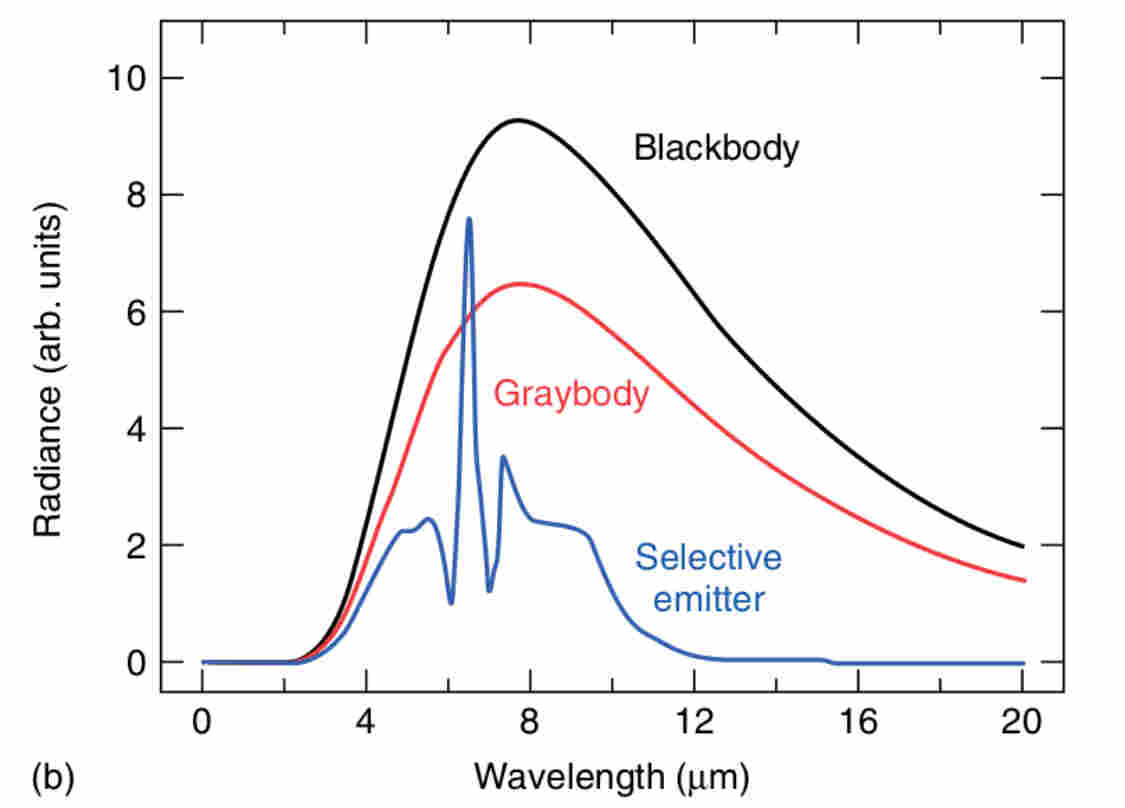
\includegraphics[scale=0.4]{Figures/Chapter01/BlackAndGreybodyComparison.jpg}
			\caption{Relationship between the blackbody spectral radiation, the radiation emitted by a grey body and a selective radiator at the same temperature. It can be seen how the blackbody yields the maximum radiance at any given wavelength.}\label{fig1.4}
		\end{figure}
		
		\bigskip
		The emissivity of real objects, however, varies with respect to wavelength and therefore they cannot be considered grey bodies. In fact, it might also depend on many other factors such as temperature and viewing angle, as we will discuss later. However, it is usually assumed that for short wavelength intervals, the emissivity can be considered constant. This assumption is used to treat real objects as grey bodies in order to avoid the associated mathematical complications of emissivity estimation. For this reason, surface emissivities are often computed as the average of the emissivity through the wavelength interval in which the infrared sensor works. This average is also possible because the emissivity is a slow-varying function of wavelength for solid objects. However, this does not apply to other cases, such as gases or liquids.
		
		A good illustration of the effect of emissivity in the measurement of the real temperature of a surface is presented in Figure \ref{fig1.5}. This corresponds to the so-called Leslie’s Cube. Even though this cube is filled with hot water and all the faces are at the same temperature we can see a huge difference in the temperature measured by the IR sensor. This is due to the difference in emissivity of the two front faces. One is painted with a high emissivity black (could be any color) paint and therefore the apparent temperature is closer to the real temperature of the water, while the other face has low emissivity (very reflective) and the apparent temperature is almost entirely due to the reflected component (see the heat from the hand reflected in the surface).
		
		\begin{figure}[ht!]
			\centering
			\captionsetup{justification=centering,margin=2cm}
			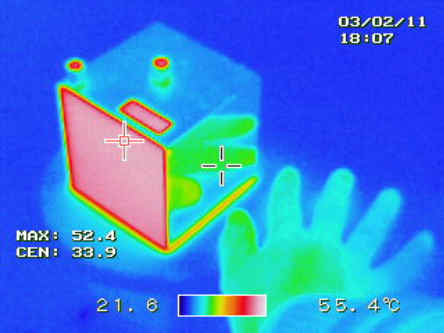
\includegraphics[scale=0.55]{Figures/Chapter01/LesliesCube.jpg}
			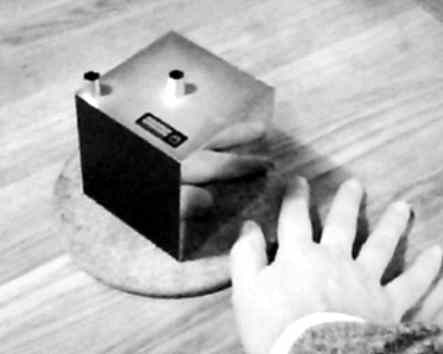
\includegraphics[scale=0.52]{Figures/Chapter01/LesliesCube2.jpg}
			\caption{Infrared (Left) and visible (Right) images of a Leslie’s cube. The cube is filled with hot water and all the faces are at the same temperature. However,  one of the faces is coated with a high emissivity paint (black) and the other has been polished (low emissivity).}\label{fig1.5}
		\end{figure}
		
		If a blackbody is surrounded by an isothermal black enclosure of the same temperature, then, in thermodynamic equilibrium, such blackbody will absorb 100\% of the radiation emitted by the enclosure ($\alpha=1$). At the same time it will emit 100\% of its own thermal radiation since it has $\varepsilon=1$. Under those circumstances, the following relationship holds:
		
		\begin{equation}\label{eq1.5}
			\alpha \equiv \varepsilon
		\end{equation}\bigskip	
		
		This is known as the Kirchhoff’s law of thermal radiation. This law, intuitively derived for the special case of the blackbody, also applies to non-blackbodies and basically tells us that the emissivity and absorptivity of any material are equal at any specified temperature and wavelength. Thus, we can rewrite Equation \ref{eq1.2} as:
		
		\begin{equation}\label{eq1.6}
			\varepsilon + \rho + \tau = 1
		\end{equation}\bigskip	
	
		And for the case in which transmissivity $\tau=0$, this becomes:
		
		\begin{equation}\label{eq1.7}
			\varepsilon = 1 - \rho
		\end{equation}\bigskip	
	
	\section{IR measurements calibration.}\label{section1.4}
	
		Usually, when we take an IR picture of an object, at room temperature for instance, we intuitively expect the entire image to be of only one color (corresponding to the ambient temperature). However, this is rarely the case. It is important to point out the fact that the IR sensor/camera does not gives us the “real” temperature values but rather an “apparent” one. We refer to these temperatures as \textit{apparent temperatures} since it’s necessary later on to correct them due to the presence of several factors that provoque deviations in what the IR sensor perceives. The most important ones can be classified as follows:

		\begin{enumerate}[label={\arabic*.}]
			\item \textbf{Intrinsic object properties}: emissivity, reflectivity, transmissivity and polishing of the surface.
			\item \textbf{IR sensor properties}: Spectral Response Function of the IR camera in the wavelength range in which it operates.
			\item \textbf{Other factors}: ambient conditions (temperature, RH), apparent reflected temperature and viewing angle of the IR camera with respect to the object.
		\end{enumerate}
		
		To understand how all these factors come into play we can consider the situation depicted in Figure \ref{fig1.6}.  Let's assume that we have a target which is placed in front of a generic IR sensor. We are interested in measuring the amount of radiation coming from the target due to emission alone, since this corresponds to the only measure of the “real” temperature of our object. Using Equation \ref{eq1.4} we can estimate the amount of emitted IR radiation ($N$) as: 
		
		\begin{equation}\label{eq1.8}
			N(\lambda,T)=\varepsilon(\lambda,T) \cdot N_{b}(\lambda, T)
		\end{equation}\bigskip
		
		Here $T$ is the actual (real) temperature of the target.
			
		\begin{figure}[ht!]
			\centering
			\captionsetup{justification=centering,margin=2cm}
			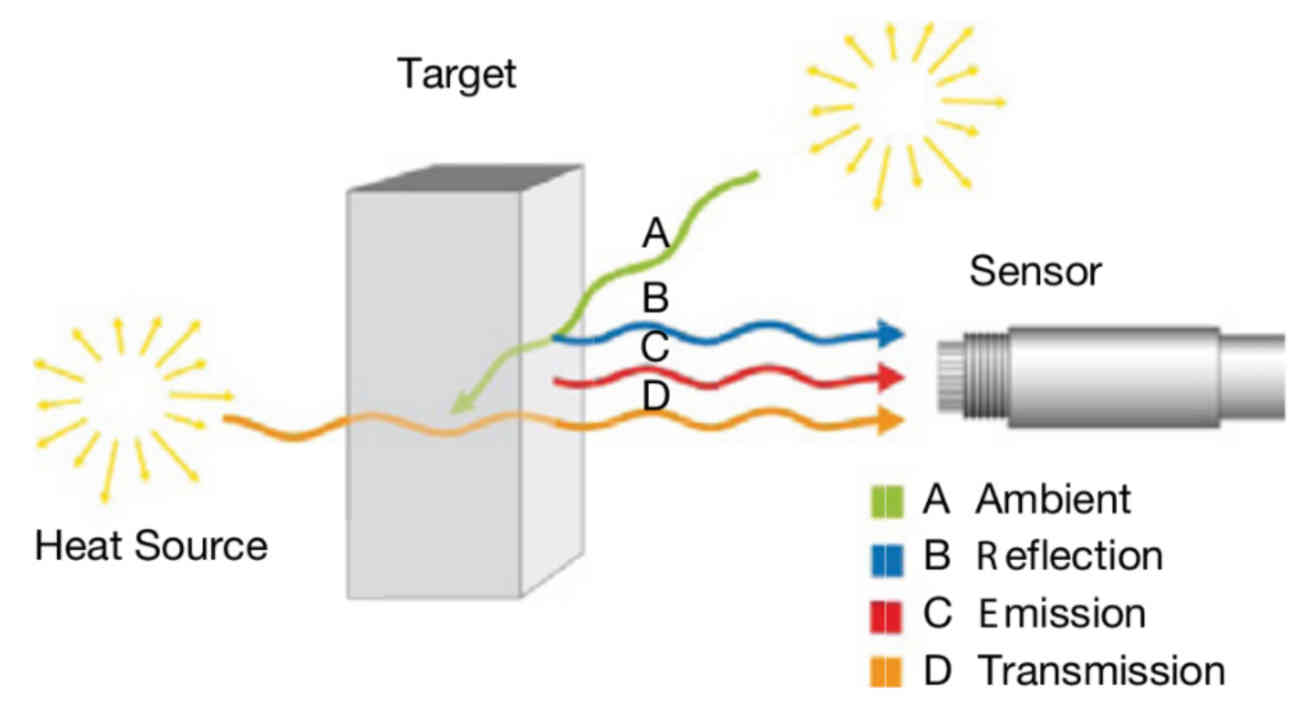
\includegraphics[scale=0.38]{Figures/Chapter01/SchematicsOfIRRadiation.jpg}
			\caption{Schematics of the IR radiation interaction with a target surface: (A) radiation from an external source being partially absorbed by the target, (B) part of the radiation from A which is is reflected in the direction of the IR camera, (C) thermal  radiation emitted from the target and (D) external source of radiation transmitted through the target.}\label{fig1.6}
		\end{figure}
		
		In addition, we will have two more contributions to the amount of IR radiation flying in the direction of the sensor. These other contributions are produced by additional sources of heat. The first is the amount of radiation coming from external heat sources that is reflected on the target surface. This contribution is given by:
		
		\begin{equation}\label{eq1.9}
			N_{ref}(\lambda,T)=\rho(\lambda,T) \cdot N_{b}(\lambda, T_{r})
		\end{equation}\bigskip
		
		Where $T_{r}$ is the \textit{apparent reflected temperature} of the target surface. This is an irreducible source of IR background, even with an isolated thermal chamber, and is therefore always present in the estimation of the real surface temperature. In this sense, we can regard the interior walls of the isolation chamber (and all other equipment inside) as “external” heat sources and, as the temperature of such objects should be close to the room temperature, this apparent reflected temperature is often taken as the ambient temperature. We will discuss further on this temperature and its estimation method in Section \ref{section3.1}. The second source of additional IR radiation is that part of the radiation coming from a heat source behind the target that is transmitted through the target itself. This contribution is determined as:
		
		\begin{equation}\label{eq1.10}
			N_{trans}(\lambda,T)=\tau(\lambda,T) \cdot N_{b}(\lambda, T_{t})
		\end{equation}\bigskip	
		
		where $T_{t}$ is the \textit{apparent transmitted temperature}. This source of IR background can be avoided by placing the target in a thermal enclosure (chamber), leaving all external heat sources outside. However, for complex objects composed by layers of different materials, this factor can appear if, for example, the surface material (facing the IR sensor) is somewhat transmissive and the heat from other layers reaches them and passes through.
		
		The combination of all these three factors is then the total amount of IR radiation coming from the target that heads towards the camera:
		
		\begin{equation}\label{eq1.11}
			N_{total}(\lambda,T)=N(\lambda,T)+N_{ref}(\lambda,T_{r})+N_{trans}(\lambda,T_{t})
		\end{equation}\bigskip
		
		Neglecting the transmission component (assuming the object opaque), Equation \ref{eq1.11} becomes:
		
		\begin{equation}\label{eq1.11a}
		N_{total}(\lambda,T)=N(\lambda,T)+N_{ref}(\lambda,T_{r})=\varepsilon(\lambda,T) \cdot N_{b}(\lambda, T)+[1-\varepsilon(\lambda,T)] \cdot N_{b}(\lambda, T)
		\end{equation}\bigskip
		
		where we have used Equation \ref{eq1.7} to express everything in terms of emissivity. If we also consider that this $N_{total}(\lambda,T)$ is not attenuated in the air path to the IR sensor\footnote{{\footnotesize We can see from Figure 1.2 (for 10 m) that the air transmissivity is nearly 1 in the LWIR region of the IR spectrum. Additionally, as we will see later on, our experimental setup was maintained at low humidity to further improve the transmissivity of the environment.}} then the emissive power at temperature $T$ registered by the sensor for a given wavelength is:
		
		\begin{equation}\label{eq1.12}
			N_{meas}(\lambda,T)=R(\lambda) \cdot N_{total}(\lambda,T)
		\end{equation}\bigskip
		
		where $R(\lambda)$ is a correction scale factor introduced to account for the fact that our IR camera is sensitive only in the spectral range from 7.5 $\mu$m to 14 $\mu$m, and even in that range it’s also not 100\% sensitive to the incoming radiation. It is often called sensor’s \textit{Spectral Response Function} or sensor’s \textit{Filter Function} \ref{ref7}. Note that this factor only depends on the IR sensor’s “efficiency” for a given wavelength and it can be estimated as the ratio of the power registered by the sensor and the power calculated using Equation \ref{eq1.12}.
		
		To obtain then the total (integrated over all wavelengths) signal processed by the IR sensor we have to integrate Equation \ref{eq1.12} over the wavelength range that our sensor is sensitive to (from $\lambda_{1}$=7.5 $\mu$m to $\lambda_{2}$=14 $\mu$m):
		
		\begin{equation}\label{eq1.13}
			N_{meas}(T)= \int_{\lambda_{1}}^{\lambda_{2}} N_{meas}(\lambda,T) d\lambda = \int_{\lambda_{1}}^{\lambda_{2}} R(\lambda) \cdot N_{total}(\lambda,T) d\lambda
		\end{equation}		
		
		\begin{equation}\label{eq1.14}
			N_{meas}(T)= \int_{\lambda_{1}}^{\lambda_{2}} R(\lambda) \cdot \varepsilon(\lambda,T) \cdot N_{b}(\lambda,T) d\lambda + \int_{\lambda_{1}}^{\lambda_{2}} R(\lambda) \cdot [1- \varepsilon(\lambda,T)] \cdot N_{b}(\lambda,T_{r}) d\lambda
		\end{equation}\bigskip	
		
		As we don’t know the functional form of $R(\lambda)$ or $\varepsilon(\lambda,T)$ with respect to $\lambda$ we can come around this by applying the integral mean value theorem and use their averaged value instead. Since both $R(\lambda)$ and $\varepsilon(\lambda,T)$ should be slow-varying functions of the wavelength, there must be certain value $\xi \in [\lambda_{1},\lambda_{2}]$ such that we can then express Equation \ref{eq1.14} as:
		
		\begin{equation}\label{eq1.15}
			N_{meas}(T)= R(\xi) \cdot \varepsilon(\xi,T) \cdot \int_{\lambda_{1}}^{\lambda_{2}} N_{b}(\lambda,T) d\lambda + R(\xi) \cdot [1- \varepsilon(\xi,T)] \cdot \int_{\lambda_{1}}^{\lambda_{2}} N_{b}(\lambda,T_{r}) d\lambda
		\end{equation}	
		
		\begin{equation}\label{eq1.16}
			N_{meas}(T)= R \cdot \bar{\varepsilon} \cdot I_{1}(T) + R \cdot [1- \bar{\varepsilon}] \cdot I_{2}(T_{r})
		\end{equation}\bigskip
		
		where $\bar{\varepsilon}=\varepsilon(\xi,T)$ is the averaged emissivity in the wavelength region in which the IR camera is most sensitive and $I_{1}(T)$ and $I_{2}(T)$ can be calculated numerically:
		
		\begin{equation}\label{eq3.10}
			I_{1}(T)=\int_{\lambda_{1}}^{\lambda_{2}} N_{b}(\lambda,T) d\lambda
		\end{equation}
		
		\begin{equation}\label{eq3.11}
			I_{2}(T)=\int_{\lambda_{1}}^{\lambda_{2}} N_{b}(\lambda,T_{r}) d\lambda
		\end{equation}\bigskip
		
		$R(\xi)$ can also be treated as a constant scale factor ($R$) which only depends on the IR sensor (See results in Section \ref{section4.4}).
		Even though we can assume emissivity as a constant that only depends on the specific material of the surface under investigation, in general, it also depends on the viewing angle of the camera with respect to the normal of the surface. blackbodies behave like perfect isotropically diffuse emitters, that is, for any surface emitting radiation, the radiance of the emitted radiation is independent of the direction into which it is emitted \ref{ref8}. However, real surfaces, in addition to the lower emission rate (given by lower emissivity) also show angular dependence in the emissive power (Figure \ref{fig1.7} left).
		
		\begin{figure}[ht!]
			\centering
			\captionsetup{justification=centering,margin=2cm}
			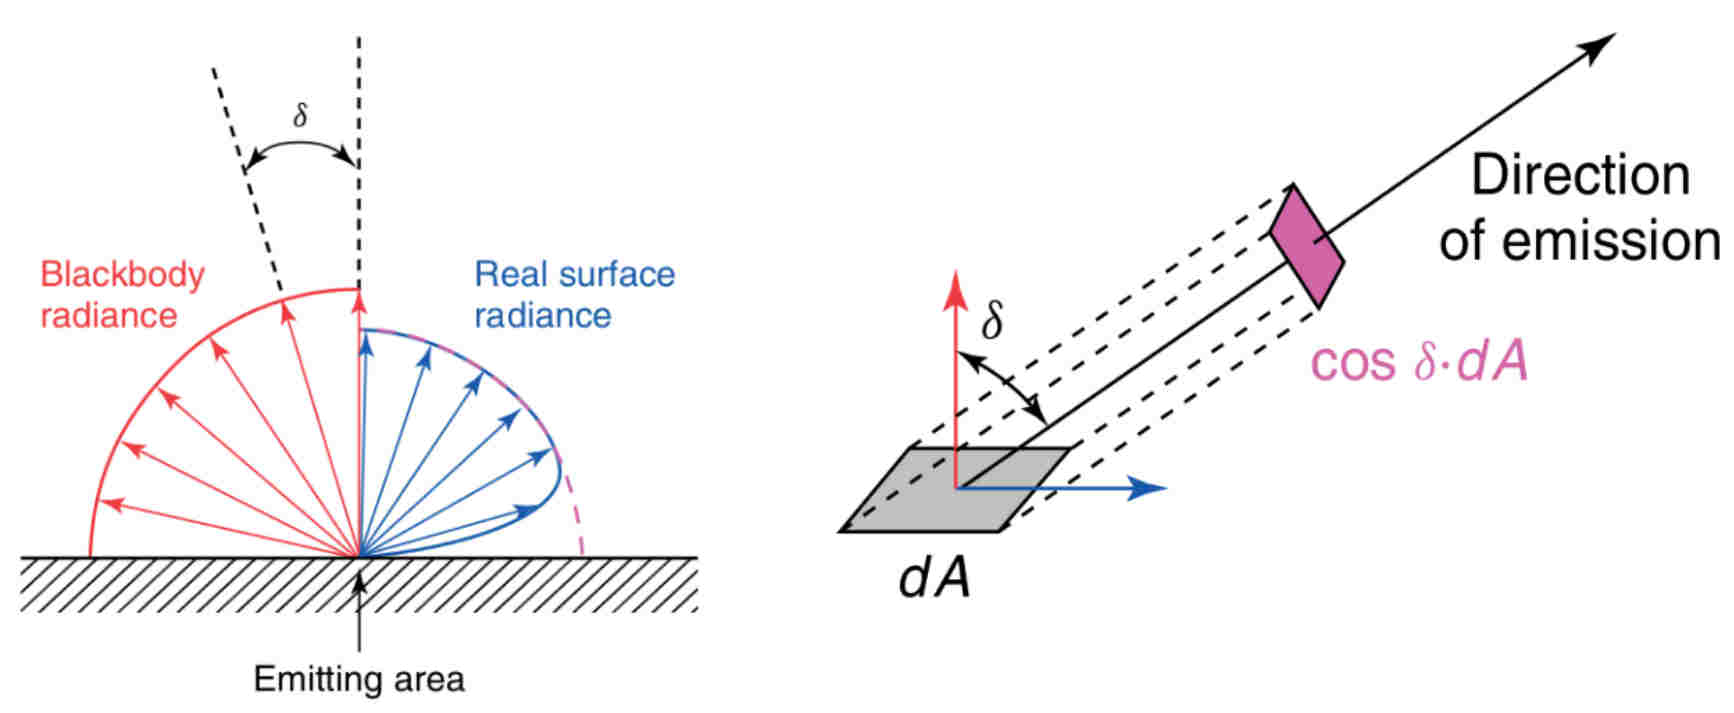
\includegraphics[scale=0.35]{Figures/Chapter01/AngularDistributionSchematics.jpg}
			\caption{Schematics of the angular dependence of the emissive power of a surface in relation to the blackbody.}\label{fig1.7}
		\end{figure}
		
		Depending on the surface, the intensity of the emitted radiation can be approximated with a cosine law with good approximation. However, in general, this is not the case, and in most cases a study must be carried out to estimate the angular dependence of the emissivity.
		